\documentclass{article}
\usepackage{amsmath}
\usepackage{bm}
\usepackage{graphicx}
\usepackage[utf8]{inputenc}
\newcommand{\myvec}[1]{\ensuremath{\begin{pmatrix}#1\end{pmatrix}}}
\title{Assignment 1}
\author{D V K M Rishab, AI20MTECH14004 }
\date{September 5, 2020}

\begin{document}
\maketitle
\section*{Assignment 1}
Solution: 
\newline \newline
\begin{math}
\bm{\vec{P}} = \myvec{7\\6} \newline \newline \newline
\bm{\vec{Q}} = \myvec{3\\4} \newline \newline \newline
A \hspace{0.1cm} vector \hspace{0.1cm} on \hspace{0.1cm} the \hspace{0.1cm} X-axis \hspace{0.1cm} \bm{\vec{X}} \hspace{0.1cm} is \hspace{0.1cm} equidistant \hspace{0.1cm} to \hspace{0.1cm} both \hspace{0.1cm} \bm{\vec{P}} \hspace{0.1cm} and \hspace{0.1cm} \bm{\vec{Q}}. \newline \newline
Need \hspace{0.1cm} to \hspace{0.1cm} find \hspace{0.1cm} k. \newline \newline
Let \hspace{0.1cm} \bm{\vec{X}} = k\myvec{1\\0} \hspace{0.1cm} be \hspace{0.1cm} the \hspace{0.1cm} vector \hspace{0.1cm} on \hspace{0.1cm} the \hspace{0.1cm} X-axis. \newline\newline\newline
\implies \hspace{0.1cm} \myvec{1 & 0} \hspace{0.1cm} \bm{\vec{X}} = k \newline\newline\newline
Also, \hspace{0.1cm} \bm{\vec{X}} = \frac{\bm{\vec{P}+\vec{Q}}}{2} \newline\newline\newline
\implies \bm{\vec{X}} = \frac{\myvec{7\\6}+\myvec{3\\4}}{2} \newline\newline\newline
\implies \bm{\vec{X}} = \myvec{5\\5} \newline\newline\newline
\implies \myvec{1 & 0}\bm{\vec{X}} = \myvec{1 & 0}\myvec{5\\5} \newline\newline\newline
\implies k = 5 \newline\newline\newline
Therefore, \hspace{0.1cm} \bm{\vec{X}} \hspace{0.1cm} = \hspace{0.1cm} \myvec{5\\0}\newline\newline\newline
\end{math}
\section*{Plot}
\begin{figure}[!htb]
    \centering
    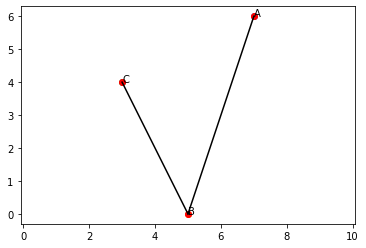
\includegraphics{Assignment1.png}
    \caption{Plot representing the Points}
    \label{Fig.1}
\end{figure}
\end{document}